\chapter{小鸡}

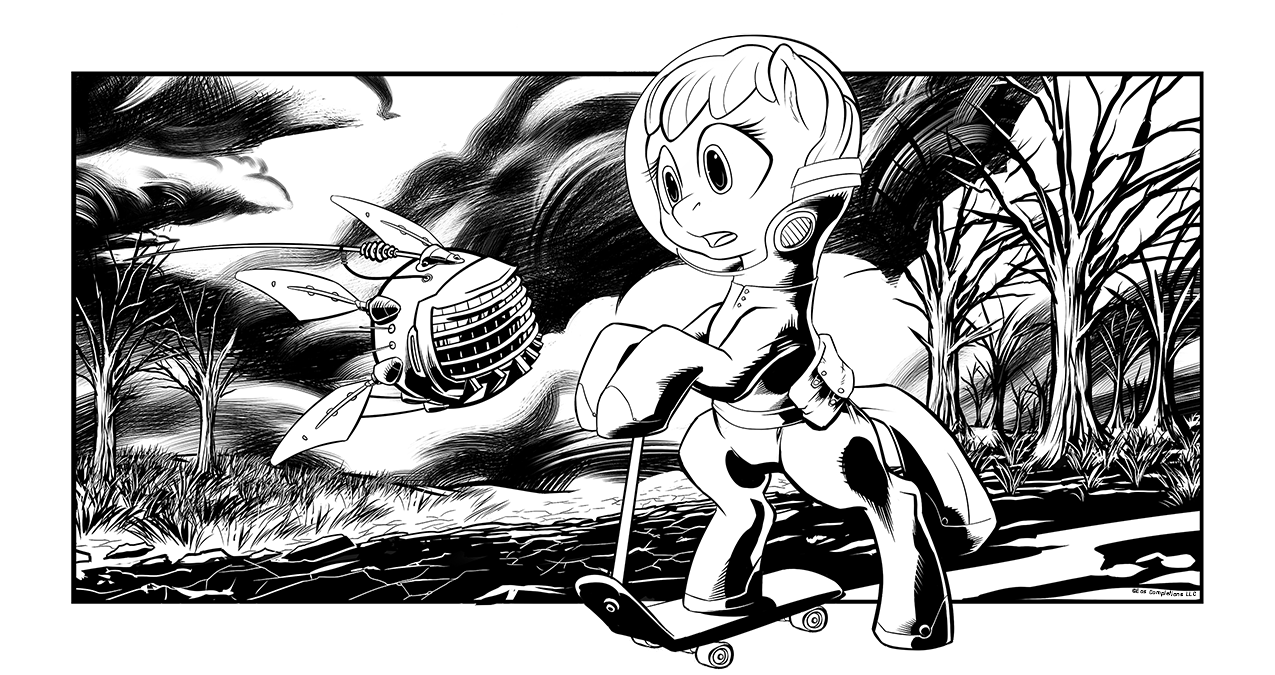
\includegraphics[width=0.9\linewidth]{image05.png}

\begin{intro}
可爱标记童子军小鸡营救队来了!
\end{intro}

\daytimeplace{5}{9:30 AM}{闹市区,盐块城}{Downtown, Salt Cube City}

「耶!漂漂牛快点!再快点!」

双头牛左边那个脑袋重重叹了口气,然后一脸绝望地望向旁边带着黑帽子的独角兽。

那小马对牛无奈地笑了笑,挥着蹄子打断她无声的抱怨:「这是交易的一部分,别不满意啦,再让这个幼驹骑最后一圈,然后带她来我办公室。」

「好,好,白先生。」牛不爽地在白塔外面转来转去,在之前的半小时她们已经跑了好几圈了。虽然外面的小马都在忙着修理昨晚冲击波造成的破坏,但是被一个黄色小雌驹骑着还是会引来很多好奇的目光和窃窃私语。

「我认得她,是嘉年华的幽灵……她诅咒了那些尸鬼,这个孩子一定会带来厄运……」

「你看,她在白塔外面装傻,我敢用我的所有瓶盖打赌,她一定用她在圆顶里面看到的东西来威胁他们呢!」

「你没看到吗?圆顶的炫彩已经消失了,然后……然后尸鬼的飞船也爆炸了!他们肯定想搞什么鬼,结果反而坑了自己。可恶的尸鬼,他们就是活该!」

「但是……她到底是谁?」

「别问,我从来没看见她吃过东西,甚至没看见她打开自己的头盔,虽然不知道怎么回事,不过她绝对不是好东西。」

「别说了,她过来了!」

帕比自己玩得很开心,完全没有去留意那些窃窃私语,「太棒了,超超超有趣,牛小姐们,我们有时间再玩一次好吗?」

双头牛的其中一个脑袋点了点头,「当然,不过你要先问问白先生,他在办公室等你,就在红色的门里面。」而另一个头一脸不爽地继续反刍着。

白先生的办公室很大,很整洁,墙上挂了很多照片,而地板亮得可以照见自己的影子。

「哇哇哇!这个地方真的超超超漂漂!」

白苹果的老大是一只戴着黑帽子的雄性独角兽,毛皮是白色,鬃毛是天蓝色。「嗯,谢谢夸奖,黛丝小姐。」这个称呼似乎让帕比愣住了,所以白先生又说:「那个圆顶的声音昨晚不是说你妈妈是阴雨·黛丝吗,所以你的全名是快乐帕比·黛丝,是吧?」

帕比歪了歪头,最后又点了点头,「嗯,没错。现在我该走了……声音小姐在我的罗盘上显示了一个箭头,所以我该往那个方向走了。我可以走了吗?拜托。」

老白叹了口气,压低帽子挡住了他的眼睛。「当然,没问题……但是……我还是想问你最后一件事情。圆顶里面以前是什么东西在发光?」

「你是说盐块吗?」帕比就像听到什么有趣问题而咯咯笑起来。「你好笨哦,我是说,你不是一直住在盐块城嘛,你居然都不知道盐块,真是……」

那个老马正要大声训那个小雌驹,但是仔细想想和小孩子闹脾气又没什么用,所以他只是笑了笑。「我承认我一直没去过圆顶,那里有点……可怕,所以,是尸鬼把那个盐块带上他们的飞船了吗?」看着幼驹一脸迷茫,于是他补充道。「就是那能飞的气球。」

帕比点了点头。「没错!他们看起来超级着急的样子!他们都说会什么……盒爆?……核包……啥的?」帕比看起来不是很开心的样子,「反正是什么什么东西,我记不太清楚了,但是他们说他们要在发生之前走得远远的,因为很危险?」

「核爆?是这个吗?」

「对!他们说因为链啥反应……反正就是那个方块要赶紧丢得远远的,我还帮他们了!」

蓝色鬃毛的小马一脸惊讶,「他们……想要带着那炸弹走得越快越好?我……我知道那些尸鬼都是疯子,但是他们居然……好吧……我想这解释了为什么圆顶的光消失之后放射性几乎消失了。」

白先生露出放心的笑容,「你干得很好,小家伙,我很想再招待你一会儿,但是你这么急着走的话,至少让我送你出门。」

「好的好的!白先生!拜拜!我会告诉我妈妈你对我很好!」

「好,一路顺风小家伙,很抱歉我有些好奇,你想去哪?」

帕比指着南边说:「那里!妈咪就在箭头的终点!」

「哦,直接去沼泽地啊……祝你好运!」

她死定了。

这个沼泽是52号国道北边最危险最糟糕的区域。这个幼驹只会变成某个废土强盗的早餐。虽然很可惜浪费了这么好的防辐射服,但是白苹果家族不是强盗。

白先生沉思了一会,回忆着昨晚的事情,虽然这小姑娘就要走了,但是这样利用一个小孩子,让他后悔不已。她或许拯救了整个盐块城,但是他又给了这个孩子什么回报呢?只是骑着牛跑两圈?她就要遭遇危险了,而他甚至连一点建议都没有?这太不公平了。

「喂!黛丝小姐!等一等!我有东西送给你!」

\horizonline

\daytimeplace{5}{11:30 AM}{盐块城外,52号国道北部}{Salt Cube City Outskirts, Big 52 N Branch}

「呀……呵……!」一颗踩着红色滑板车的黄色子弹飞驰在公路上。

盐块城的建筑早已远远甩在脑后,路边的景象又变成了一片荒芜的废弃农田。

% NOTE: 遵照英文发布版改

\rcpr{仔细听我说,你到了乐麦镇之后,就绕道,穿过沼泽的路——}怎么怎么怎么怎么\rcpr{——一定要记住,绝不要穿过}什么什么什么……一些无聊的东西,帕比已经记不清了!

幼驹骑着滑板车嗖嗖地飞驰向南方,似乎是觉得滑板车的声音不够刺激,帕比还自己加上音效。「呜呜……嘟嘟……!飞向月球!宇宙无限!太空战士安德洛队长拯救世界!耶!」

在黄色幼驹面前,路上都是腐烂的田地和荒芜的农场,盯着箭头走了一会之后,农田变成了枯萎的果林和满是泥水的水坑。偶尔会有一两个营地,但是看起来已经遗弃很久了。虽然还有一点点生命迹象,但是都是一些昆虫或者不敢惹帕比的野兽。

唯一敢于接近帕比的,是一个飘在路中间的机器精灵。

「嘀嘀,我是吉普车!太空战士来啦!」帕比在玩疯的时候从来不会注意细节,黄色子弹继续以最高速度飞驰着。机械精灵在被撞上的前一瞬间连忙躲开,然后又急忙追着帕比飞。

「嗨,帕比,这么急着去哪儿啊?」一个熟悉的声音从喇叭里面传出来。

「提问者!我好想你!快看我的新滑板车!」帕比一边全速前进一边咯咯笑着,「我还认识另一个说话机器,不过那个很有趣,或许她不是一个机器?我不确定。」

「真有趣,可以和我讲吗?」机器精灵没等回答就接着问。「昨晚盐块城发生了什么?那个大爆炸是怎么回事,圆顶怎么了?你能停一下么,拜托!」

帕比叹了口气然后开始减速。「真会挑时候,人家正玩得开心呢……」

停下来之后,幼驹跳下滑板车,她一边想着守望者的问题,一边敲着头盔下面下巴的位置。「你是问圆顶?我在那里交了好多朋友!老大沙盒,软气先生,桃花小姐……哦哦,还有声音小姐!」

「不是声音先生了?」

「不对,傻机器,有一个声音先生,还有一个声音小姐!她住在圆顶但是声音先生可以随时叫她来,她超级酷而且帮我给尸鬼们办了一个送别派对!」

「哦,另一个小马--机器智能交互界面么……那么……你见到了尸鬼,还办了一个送别派对?你是什么意思?你帮他们发射的飞船?」

「太对了!」帕比兴奋地点着头。「超超超超级棒!我从窗口看到一个大大大大的东西高高高高地飞上天!」帕比举起前蹄描述那东西飞得多高,但是举过头了让自己一屁股坐在了地上,她咯咯笑着坐正了继续说。「然后好多好多灯照得雪亮雪亮的!我听到我的声音超超超超级大,所以我说『啦啦啦……拜拜尸鬼』然后他们就飞走啦!超级酷!滑板酷!」

「滑板什么?」

「滑板酷!」

「有这说法吗?」

「当然滑板!」

「你知道么……显然那滑板对你的小脑袋没什么好处……」守望者的声音听起来有点担心,「好吧,扯远了,那爆炸是怎么回事?」

「什么爆炸?」帕比不解的歪着头。「你说房顶又塌了?」

「不是,我是……等等……又有房顶砸你脑袋上?」这句话很明显让守望者有些惊讶。

「没错,那个房顶打开,然后大气球飞走之后,整个地方嘎吱,然后咣当!正好掉我头上。」帕比咯咯笑着,「但是我是一个超级太空小马,所以我把自己挖出来了……我就是那么厉害!」幼驹自豪地笑着。

机器的喇叭里面传出一阵笑声,然后又是一个叹息。「好吧,现在你要去哪儿?」

「当然是下一个妈妈地点!很明显,第三次会交好运!」

乒!乒!

忽然一阵枪声在空中响过,不过子弹明显不是向着帕比或者守望者来的,但是幼驹很明显听到了声音。「那是啥?」

「我……很抱歉帕比,我该走了,附近可能有强盗,你最好躲起来等他们火拼结束。」

「火烧?哪有?我要吃!」帕比蹦蹦跳跳地四处张望起来。

「塞拉斯蒂娅公主,请务必保佑她安全……」机器精灵的声音被一阵音乐代替之后,那个无人机飞走了。

声音是从帕比头上传来的,小幼驹抬头看的时候,看到令她难以置信的景象:有些超级大的飞天小马一边放着烟花一边飞来飞去,就像超华丽的芭蕾舞。这个场景让帕比回想起那天妈妈带她去飞行场看漂漂天马在天上做超级有趣的表演。

这次看起来也差不多,虽然有点不同的是飞在天上的小马不停地在闪光并且发出很大响声,帕比马上觉得这一定是他们最喜欢玩的娱乐项目。

但是她马上发现那些大家伙不是天马,所以幼驹皱着眉头问道:「我说,声音先生……那些小马生病了吗?」

「{\mtzh 分析中。友善的狮鹫。}」

虽然帕比一点都不明白狮鹫是什么,但是如果声音先生说那是『友善』,那么都可以啦。黄色幼驹挥着蹄子大喊起来。「喂!漂漂马!我在这里!喂喂!」

其中一个生物转头看了地面一眼,然后放松警惕的它马上就被另一个生物击中,然后打着转栽了下来。

「呃……我看看……一……二……三……呃……」帕比想数一数有几个狮鹫,但是他们飞得太快,所以她还是跑向那个倒在地上的家伙身边,幼驹注意到她根本不是小马,看起来像是某种半鹰半狮的奇怪生物——她觉得那东西看起来真滑稽。

「我说,小鸡先生!」

那生物一动不动,一大滩血正在他身体下面慢慢扩展,帕比用蹄子戳了他一下。「喂,怎么啦?」

没有反应。

「呃,小鸡先生?起床啦?太阳高高哦!」

依然没有任何反应,这看起来可不太妙。不过最糟糕的是他的朋友似乎根本没注意到这边的情况,所以她该做点什么。

「喂!小鸡们!你们朋友受伤了!快下来啊!」帕比用自己最大声音,挥舞着双蹄大喊着,但是很明显她被忽略了。那剩下的三只狮鹫还在天上跳着华尔兹,不断有血从天上洒落到她头上。

「唉,他们玩得太开心不理人家!」帕比叹了口气。「如果我能有什么东西吸引他们注……等等,我有!」幼驹微笑的想起那个白先生给她的那个闪闪东西,那叫什么来着,揪毫民?九耗毛?「呃……声音先生,给我那个闪闪发光还很聒噪的东西!」

「{\mtzh 警告,物品『快乐帕比』不能从物品栏中取出。}」

「喂喂!你这样不对吧!你知道我说什么!那东西,那个揪毫毛什么的!白先生给我的那个!」

「{\mtzh 肯定,取出『九毫米半自动手枪』。}」

枪飞到了帕比面前。幼驹把这个铁块握在蹄子上举向天空。「喂!喂喂!喂喂喂喂!听我说啊!这东西怎么用?怎么发出声音?」

「{\mtzh 读取介绍中……射击模式『危急时刻』!首先,将枪指向目标,然后,说出『开火』或者『啪』,枪就会击发。如果想要装填的话,将武器放入物品栏再取出即可。}」

「呃,听起来超简单。」帕比指着狮鹫,「啪!」

乒……

% NOTE: 呯 -> 乒

「哎呦!」

后坐力让枪从帕比蹄子上飞出,砸在她头盔上让她坐了一个屁股蹲,然后落在了不远处。

其中一个狮鹫痛得大叫起来。「见鬼!他有后援!杀了那个傻……」他还没说完,他的头就爆成了一团血雾。现在天上只剩下了两只狮鹫,战斗变成了一对一的厮杀。

两只狮鹫冲撞在一起,用喙和爪子又撕又咬,帕比走到那个落下来的狮鹫身边,看到他的头不见了。「你知道吗,声音先生……我觉得他们不是在玩。这个小鸡……呃……死了?」

「{\mtzh 肯定。}」

「呃……嗯……」帕比皱起眉头。「另一个呢?」帕比指着地面说:「他也死了?」

「{\mtzh 分析中,没有生命特征。目标已死亡。}」

帕比又看向天空那俩纠缠在一起的狮鹫。「他们俩……在相互伤害对方?」

「{\mtzh 肯定,每一条线索都表明他们在死斗。}」

「好吧……」帕比想了想,然后说:「我怎么让他们停下呢?哦,我有点子了!」帕比深吸一口气:「拜托请别打架了!某马会受伤啊!」

实际上某马已经受伤了,或者说,某狮鹫,但是帕比并不太清楚幸存的俩斗士什么情况,他们似乎完全没有注意帕比,但是其中之一忽然发出一声尖叫,然后他们一起打着转从天上栽下来。

帕比跳上滑板立刻追了过去,想看他们落在哪里,等她到那里的时候,看到其中一只狮鹫胸口被抓开,喉咙也有一个血窟窿,而另一个尝试站起来的狮鹫身上的好几个伤口都在流血。

「小鸡先生,你还好吗?」幼驹飞奔到那个想要站起来的狮鹫身边,但是他却倒在了地上咳嗽着。「你看起来不太好。」

「咳咳……你就是开枪的那个……谢谢……」

帕比皱了皱眉,「我……是啥?」

「咳……咳……听我说……我……我女儿……在……南边……军营……咳咳……」狮鹫痛苦的喘息着,「赫瑞塔……她……在那等我……咳咳……求你……去……把这个……给她……」狮鹫递给帕比另一只枪,这支枪比她的那一把重多了,而且表面是全黑的,枪口还有一条红线装饰。

% NOTE: ignore overfull

「呃……好的?」帕比戳了戳狮鹫,「没问题……但是……你会好起来吧……是吧!」

「你……你是笨还是……我要死了……」他咳出一口血打断了他的话,「告……告诉……赫瑞塔……我……我要她……往南……告诉她……我…………我……告诉……」随着最后一丝光芒从狮鹫眼中消失,他的声音也同样消失了。

帕比等了一会,然后又用蹄子戳着狮鹫,「嘿,小鸡先生,你睡着了?小鸡?」她又戳了戳他。「呃……我想……我该走了……我……呃……很抱歉……」幼驹从死去的生物前后退了一步,她感觉很糟糕,有什么东西完全不对。虽然不是第一次看到死去或者正在死去的生物,但是……她从来没有像这样仔细注视过。

如果说现在是个证明「这个世界上小马都是相互杀害对方而求生」的好机会的话,对于帕比来说这只是个伤心的故事。

「呃……我希望你能好起来,不过现在我真的……真的真的……要走了,抱歉……」幼驹透过头盔吻别狮鹫之后。跳上她的滑板跑远了。

「声音先生,你在吗?」

「{\mtzh 肯定,系统一切正常。}」

「为什么漂漂小马都要互相伤害?」幼驹皱眉问。

「{\mtzh 警告,该程序并没有社交功能。}」

帕比叹了口气继续顺着粉色箭头往前走。「呃,声音先生……那个小鸡说什么女儿的事情?」

「{\mtzh 肯定。已经被设为次要任务目标:坏消息,新伙计。}」

帕比犹豫了一会之后停下滑板车说:「你能告诉我她在哪吗?」

「{\mtzh 肯定:赫瑞塔·火红(Henrietta Firebright)设为新的目标地点。}」

帕比看了看那消失然后又出现在同一个方向的粉色箭头。「呃……我觉得没设对吧?」

「{\mtzh 否定,新目标已经正确校准。}」

帕比叹了口气,操作这个奇奇妙妙的太空服是声音先生的工作,如果他说没问题,那么就没问题。

「我们走。」

\horizonline

\daytimeplace{5}{14:00 PM}{165战指附近,盐泥沼泽}{165Th Brigade field Headquarter, Salt Marshes}

「{\mtzh 警告,密封多处破损。警告,罗盘失灵。警告,无线电离线。警告,医疗系统离线。警告,头盔破损。警告,粉色药剂发现。维修回路启动。}」

「呃……我觉得……我是不是踩到什么了……」帕比想站起来但是又摔倒了。「晕晕乎乎……」

在幼驹面前的一堆路标写着『注意,雷区』和『军事管制区,禁止通行』在她身边落了一大堆沥青碎片,而她面前的路面少了一大块。不过那个滑板车却奇迹一般倒在幼驹身边,毫发无伤。

「唔……声音先生,为什么路面嘣地炸了?」她身上的每一个破洞都包裹着粉雾。

「{\mtzh 分析中,爆炸原因是地雷。无线电恢复,头盔修复。}」

帕比皱了皱眉头,「什么是地雷?等等!你总是这样!说好多听起来很厉害可是我却听不懂的话,那样我就没法因为你说错了什么对你生气了,是吧?我要专家来帮忙!叫声音小姐来!」

「{\mtzh 开启通讯连接,请稍候,罗盘恢复正常,医疗系统上线,读取目标001号个性化信息:快乐帕比,目标已死亡,状态稳定,完毕。}」

不到五分钟防护服就完全修理完了,修理用的基本都是帕比捡进口袋的各种垃圾,幼驹对她身上装的东西没什么选择性,只要五颜六色还闪闪放光就捡起来,而自我修复魔法也没什么要求,任何包括金属,玻璃,塑料的材料都可以。

「喂,喂喂?这里是盐块城圆顶紧急线路,很抱歉但是现在所有职员都已经死了,请等服务恢复以后再联系,拜拜!」

「等等,声音小姐,是我,帕比!」

「哦,帕比!你好,好久不见,你去哪了?你找到我让你找的东西了么!我的迁移协议随时准备就绪。」

「呃……没,抱歉,声音小姐,实际上,我需要帮助。」

「哦,别担心,我会在这里等你,反正都两百年了,再等几个世纪也没关系!所以,你想要啥?」

「呃,我正像神奇天马一样骑着我的新滑板……」

「等等等!你有一个新滑板?是红的?」

「那是当然的啦!」

「滑板酷!它很快,超快,还是超超超超快?」

「坐在上面就像坐火箭一样所有东西都嗖嗖往后走!你真应该试试看,超疯狂!」

「我真想试试看,你给我找个原型身体我就可以试试看,一言为定哦!」

「当然,萍琪毒誓!」帕比想要拍自己的眼睛但是被头盔挡住了。

「耶!好了,扯远了,你打电话来是想跟我炫耀新滑板的?」

「呃……不是……实际上我遇上了会爆炸的路……你看,声音先生跟我说什么地瓜啥的,但是我觉得地瓜应该很好吃而且不会爆炸。」

「哦,那取决于地瓜的品种,不过我想我知道你想说什么了,地面爆炸了而且不知道地雷在哪里……现在请你看看附近,有没有类似大号扁平飞盘而且上面亮白灯的东西,或者也可能是难看绿或者恶心黄……」

帕比笑了起来,「对对对!我看到了!等等……有好多好多!满地都是!就好像一大堆萤火虫,赞哦!」

「哦,我知道你说的地瓜是什么了,没关系,我要亲自看一下,等一下!」头盔的HUD闪了闪光之后,整个头盔都亮起了目标信号,每一个地雷的位置都标记了出来。「哇哦,四十五个,还有更多!这让我想起了我平时玩了很多很多次的那个游戏。」P7稍微顿了一下,等待整个雷区扫描结束。

「完成!现在我规划出一条路径,你只要照我说的那么走,就可以顺利到对面啦!」

\horizonline

\daytimeplace{5}{11:45 PM}{165战指附近,盐泥沼泽}{165Th Brigade field Headquarter, Salt Marshes}

这个基地看起来毫发无损,一排巨大的机库在一个大院面前,附近还有好多小碉堡,前面有一对自动防御机枪,但是一辆大号坦克压烂了它。几乎把整个大门都撞垮了,只留下一条能让一只小马勉强进去的缝隙。

帕比呆呆地看了一会,然后兴奋地爬进坦克之中。

「哇啊!这东西装满了亮闪闪的东西!瞧这个!」幼驹拿起一颗弹头有红条的炮弹,看起来很大,估计是坦克的主炮弹药。「真漂亮,喂!那还有好多!这个是黑色,还有蓝色,呦呵!」

在拆了坦克的弹药箱之后,帕比终于想起了正事。她走进基地,庭院中还有更多坦克,但基本全都丢在那里,被沼泽的湿气锈烂了,各种奇怪的植物从窗户里面冒出来,帕比似乎没看到狮鹫女儿的迹象,所以她做了她觉得最合理的事情。

「咕咕……咕咕……咕咕……咕咕……咕咕……咕咕……咯咯哒……咯咯哒……咯咯哒!」还是没反应,真奇怪。「或许她睡了?」

% NOTE: ignore overfull

「{\mtzh 警告,发现敌对生物,距离 100\,m。}」

一个巨大的生物从一所小屋里面露出头来,看起来是某种狮子,但是却大很多,而且还有一对皮膜翅膀和一条刺针上滴着毒液的长长蝎子尾巴。

「{\mtzh 分析中。蝎尾狮,威胁等级:致命。}」

「呃……那不是我要找的小鸡。」帕比转头走向那个野兽,完全不管警告。或许他知道那个女孩呢。

「嗨,我是快乐帕比!你看到我妈妈或者有个漂亮小猫尾巴的小鸡吗?」

那头巨兽低头看着小小马,嗅了嗅之后,低吼着后退了几步,看起来是被快乐帕比吓到了。

「你听到我说话了吗?拜托,超拜托!加樱桃的拜托!她有俩翅膀,一个喙,而且很小,呃……不知道她有多小,不过我想她应该很小,你在听我说话么漂漂猫猫?」

蝎尾狮吼着拍了帕比一爪子,把她打出10米多远,然后转头走进了半毁的建筑中,等在地上滚来滚去的帕比站起来之后,她对那个野兽的巢穴吐了吐舌头。「呸呸呸,坏猫!我自己找小鸡去!」幼驹皱着眉头,「真是的,这里的动物都这么漂漂,为啥小鸡要躲起来?」

帕比走进另一个看起来完好的小建筑,她探头进去。「呃,有马在吗?」她看到一面点亮的电脑屏幕,幼驹走进屋子,看到这里是个小办公室,还有几张桌子和一排柜子,在电脑上显示着一行字:「{\mtzh 请输入密码。}」

我有没有说过帕比基本上不识字?「亲……请……请是……什么?」

这回你明白了吧。

「密码?密码!我知道,我知道,快乐帕比!」

在输错几次结果电脑自动锁定之后,帕比已经对这个『写你名字』的游戏烦死了,她是肩负重任的小雌驹!好吧……是肩负很多重任,所以她要抓紧时间!没错!

虽然机库外面看起来毫发无伤,不过里面的屋顶早已经塌了,在徒有其表的外观里面剩下的只有一大堆的废墟和碎石,为了保险期间,帕比还专门在每个机库都看了看,结果除了碎石头之外什么也没找到。之后小雌驹注意到有个可爱的闪光金属盘,上面似乎有几个玻璃珠不见了,不过她不确定玻璃珠去哪了。

帕比继续搜索另一座建筑,这看起来是个观察塔,墙非常厚实,而且地面只有一个入口,还没窗户。里面的小小空间有一堆营火的残骸,一堆床垫和一些空罐头,甚至还有一张小桌,上面摆着一个坏掉的通信晶片,一堆箱子放在塔顶楼梯边。

防护服的声音忽然响了。

「目标到达,阴雨·黛丝的营地。」

「等等……你说什么?妈妈在这里?妈妈!是我,帕比!妈!妈咪!」或许她在楼上?帕比急忙走上楼梯,虽然楼梯很破旧了,但是还是能用。她顺着楼梯走到一个小屋,在屋子的四面都有控制板,大大的窗户可以看到整个基地,但是屋子空无一物。

帕比停下来看了看这个屋子。「我妈妈去哪了,声音先生,你说她在这里!为什么一直骗我!」

「{\mtzh 警告,该程序并没有社交功能。}」

「你……你你!为什么每次我想要说你,你就这么说!?你是个坏声音,你应该认错!让我和声音小姐说话,她懂我!她关心我!」

「{\mtzh 开启通信连接。}」

 P7的声音代替了防护服的内置声音。

「嗨,感谢您的来电,很抱歉职员都已经死光光了,请稍候再……」

「是我,帕比,你好,声音小姐。」

「哦,你好,帕比!你最近真能给我打电话!你觉得寂寞了吗?」

「有点……呃,但是我想问你一件事,很重要!」帕比皱了皱眉头。「妈妈在哪?」

「给我几分钟,处理数据中。处理结果,物品未找到,我很抱歉帕比,我不知道你妈妈在哪里,但是如果我没读错你的数据的话,你现在就在她最后所知地点。」

帕比皱了一会儿眉头,想要理解那些复杂的词,「呃……再说一次?可以吗?」

「你妈妈曾经在这里,但是她已经走了!或许你再找找有没有什么东西可以重新定位她。」

「但是……去哪儿了呢?」帕比已经快失去信心了,她本来很确定能在这里找到妈妈,但是这次尝试也是石沉大海,她觉得开始失去希望了。

「让我帮你好吗!好吗?你乖乖的坐好,我扫描这个区域,来,我们开始吧!你看,在控制台上有个磁盘!」

帕比走到磁盘面前然后用蹄子举起来。「这个让我想起软气给我的那个……」帕比把它接上外衣。「这东西说了妈妈在哪吗?」

「是个声音文件,或许上面录了什么,我们看看……我说这东西够老了!两百多年了!想要现在听还是一会听?」

「呃,当然是现在听!」

一个雌性声音从衣服喇叭里面传来,帕比睁大了眼睛,是妈妈的声音!终于找到她了!但是有点不对,她在咳嗽……她生病了吗?

\rspr{「第十四天……我已经用完……咳咳……辐特宁了……这个……咳咳……云看起来在动……咳咳……但是这里整个是个死亡陷阱。」}

% NOTE: ignore overfull

声音停止了一会儿,然后是有马在喝水的声音。

\rspr{「见鬼,我恨死这个世界了,恨死……咳咳……斑马还有公主……是他们把我们都害死……唯一不让我……咳咳……发疯的事情就是,至少帕比安全地呆在避难所……」}

然后又是一个长长的暂停。

\rspr{「我对不起你,我把你诞生到一个什么破烂世界啊!我……」}

雌驹的呼吸渐渐急促起来,她开始哭泣,帕比跳了起来。

「妈咪!别哭!我很好!我没事!妈妈!请不要哭!我……我是个好孩子,请不要哭了!我……我现在就回那个灰扑扑的地方,然后说你给我的咒语!请别生我的气!」

\rspr{「我……我必须坚强起来,帕比很安全,她在避难厩里面,我……咳咳……必须相信。现在,我该……看起来南边……咳咳……还有几个大城市,放射尘埃在那边会少……咳咳……但是我走了这么久……咳咳……不知道我还有没有力气……」}

声音消失了几秒,然后另一个声音文件又开始了。

% NOTE: 缺字

% \rspr{「十六天,肏蛋,虽然不咳嗽了,但是我居然尿血,我要赶紧走,要不然太迟了。」}
\rspr{「十六天,操蛋,虽然不咳嗽了,但是我居然尿血,我要赶紧走,要不然太迟了。」}

\rspr{「给派对星和软气:如果你们还活着,请听到这个录音之后向南,我向南走了。我会试着沿着52国道走到糖霜山脉的隧道口。我在那里等你们,我希望能在隧道维护室找到一些遮风挡雨的地方。或许能让我躲过辐射最严重的影响。」}

然后暂停了一下。

\rspr{「死鬼露娜!又开始下绿雪了……女神我诅咒你们全家!你们到底对小马国做了什么?这里曾经是被祝福的大地,为什么你们不在一切都太迟之前悬崖勒马!帕比……我好想你……如果能见你哪怕最后一面,我就算是死也无怨无悔了。」}

帕比蜷缩在地上,听着自己母亲的声音,她完全不知道怎么办,她母亲在南边的某个地方迷路了,而且要死了,幼驹现在就想见她母亲,想抱抱她,想告诉她自己一点事都没有,就算自己并不是一切安好。

但是,不管怎么说,帕比知道她母亲是最棒的小马,而且她一定会安然无恙。妈妈说要往南走,或许她现在就应该走了。帕比不能躲在这里等悲伤侵蚀自己的心,她还有希望!

「声音小姐,你还在吗?」

「{\mtzh 否定。通信已中断,有什么需要吗?}」

防护服的声音马上回答。

「哦,是你啊,声音先生,我……呃……我想去另一个地方,某个隧道口,在糖霜山。」

「{\mtzh 肯定,隧道镇已被设为新目标。}」一个新粉色箭头出现在头盔HUD上。

「太棒了!让我们……」

「蠢货,你敢再动一个蹄子试试看?」

一个尖嗓音打断了帕比,幼驹转头看向声音的方向,看到一个比成年飞马小一点的有翅生物。「给老娘把蹄子放在能看见的地方,然后说你在干……」

嗷呜!!!

年轻的狮鹫立刻低头滚进屋子里面,一个巨大的狮头咬到了她一秒之前所在的位置,窗户的铁架子在蝎尾狮有力的下颚一咬之下就弯曲了,然后它下一次就撑开了窗户,接着蝎尾狮整个冲了进来。

「我了个擦!吓死老娘了!快下楼!」年轻的狮鹫抓起帕比就顺着楼梯滚了下去。「这东西从哪来的?」

「呃……你好,我是快乐帕比!」虽然幼驹不太确定是自我介绍的好时候,但是妈妈从小就教育她要有礼貌。

「给老娘闭上你那臭嘴!肏你妈怎么啥鸡巴玩意儿都跑南边来了?」狮鹫躲在楼梯下面看着蝎尾狮巨大的身体卡在天井下不来,于是她掏出一柄枪管有黄条的手枪,对着蝎尾狮的脸就是一梭子。

「猫咪,给老娘乖一点!」

外面传来一阵恐怖的怒号,还有爪子抓水泥墙的声音。

「真好,太棒了,这下把它给惹急了。」

「呃……嗨……小鸡小姐?你可以放我下来么,漂漂拜托?」

「漂漂啥?老娘不是小鸡,你丫再敢说一次老娘就……」随着一阵金属被撕裂的声音,天井的入口被扯下来的控制板挡住了,蝎尾狮显然是把两个女孩困在里面,然后蹲在底层的入口前等她们现身。

「这野兽真他娘的聪明,这尼玛不公平!」

~\vfill

\begin{note}
    升级(Lv 4)

    新技能解锁:Heave Ho!——你是投掷专家,你扔的所有东西都飞得更快更远。
\end{note}



